\documentclass[12pt, a4paper]{article}

\usepackage{amsmath, amsthm, amssymb}
\usepackage{geometry}
\usepackage{hyperref}
\usepackage{enumitem}
\usepackage{xcolor}
\usepackage{parskip}
\usepackage{tikz}
\usepackage{pgfplots}
\pgfplotsset{compat=1.18}
\usetikzlibrary{arrows.meta, positioning}

\geometry{margin=2.5cm}
\hypersetup{colorlinks=true, linkcolor=blue!60!black}

\theoremstyle{definition}
\newtheorem{definition}{Definition}[section]
\newtheorem{theorem}{Theorem}[section]
\newtheorem{example}{Example}[section]
\theoremstyle{remark}
\newtheorem*{remark}{Remark}

\newcommand{\E}{\mathbb{E}}
\newcommand{\R}{\mathbb{R}}
\newcommand{\Prob}{\mathbb{P}}
\newcommand{\Leb}{\mathrm{Leb}}
\newcommand{\cL}{\mathcal{L}}

\title{\textbf{Likelihood: from first principles, v10}\\
\large The surface $f(x,\theta)$ and its two readings}
\author{B.~Garbuzov\\
{\small Technical notes, 2026}}
\date{}

\begin{document}
\maketitle
\tableofcontents
\newpage

%------------------------------------------------------------
\section{One function, two readings}
%------------------------------------------------------------

Fix a parametric family $\{f(\,\cdot\,;\theta) : \theta \in \Theta\}$
on a measurable space $(\mathcal{X}, \mathcal{A})$.
Here $f(x, \theta)$ is a function of \emph{two} variables:
the data point $x \in \mathcal{X}$ and the parameter
$\theta \in \Theta$.

\begin{center}
\renewcommand{\arraystretch}{1.4}
\begin{tabular}{llll}
\hline
What is fixed & What varies & Name & Interpretation \\
\hline
$\theta$ & $x$ & Density $f(x;\theta)$
  & How probability is spread over outcomes \\
$x$ (observed) & $\theta$ & Likelihood $\cL(\theta;x)$
  & How compatible each $\theta$ is with the data \\
\hline
\end{tabular}
\end{center}

\bigskip
\noindent
\textbf{Same function --- two perspectives.}
The surface $z = f(x,\theta)$ is a single mathematical object.
Slicing it parallel to the $x$-axis gives densities.
Slicing it parallel to the $\theta$-axis gives likelihoods.

%------------------------------------------------------------
\section{The Gaussian case: the surface in full}
%------------------------------------------------------------

\subsection{Setup}

$\mathcal{X} = \R$, parameter $\theta = \mu \in \R$
(mean), known $\sigma = 1$:
\[
  f(x, \mu)
  = \frac{1}{\sqrt{2\pi}}
    \exp\!\left(-\frac{(x-\mu)^2}{2}\right).
\]
This is a function of two real variables.  We can plot it as a
surface in 3D with axes $x$ (data), $\mu$ (parameter),
$f$ (height).

\subsection{The 3D surface}

\begin{center}
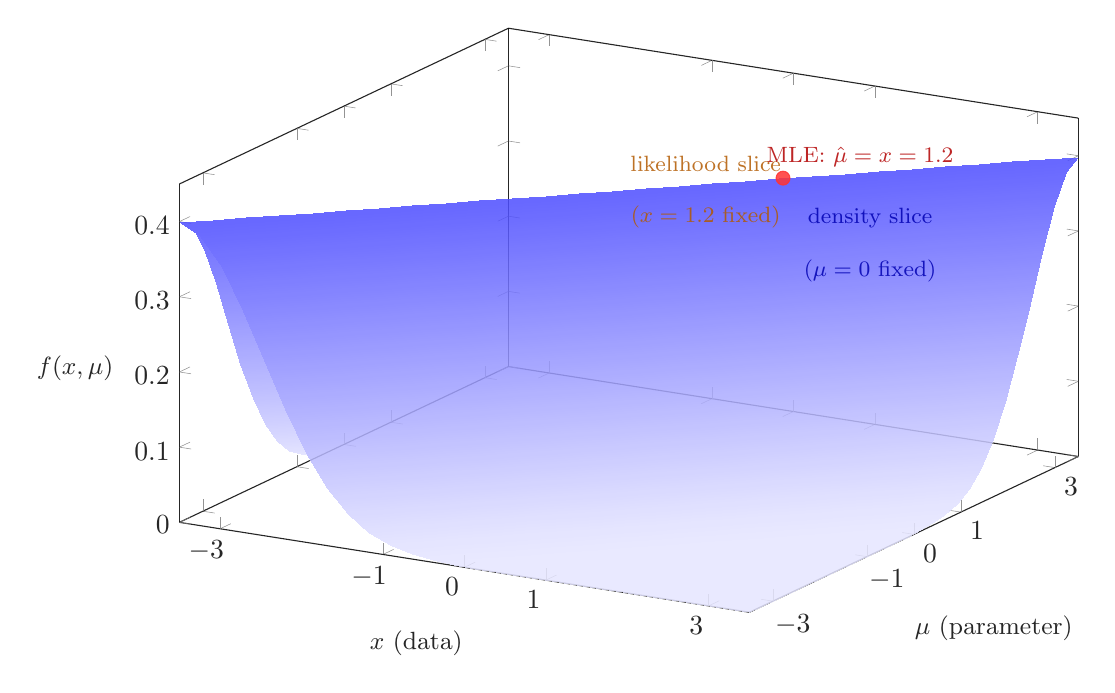
\begin{tikzpicture}
\begin{axis}[
  width=13cm, height=9cm,
  view={30}{28},
  xlabel={$x$ (data)},
  ylabel={$\mu$ (parameter)},
  zlabel={$f(x,\mu)$},
  xlabel style={font=\small},
  ylabel style={font=\small},
  zlabel style={font=\small, rotate=-90},
  xtick={-3,-1,0,1,3},
  ytick={-3,-1,0,1,3},
  ztick={0,0.1,0.2,0.3,0.4},
  zmin=0, zmax=0.45,
  colormap={blues}{
    color(0)=(blue!10!white)
    color(100)=(blue!70)
  },
  shader=interp,
  surf,
  samples=28,
  domain=-3.5:3.5,
  y domain=-3.5:3.5,
  opacity=0.85,
]
\addplot3 [surf, colormap name=blues]
  { (1/sqrt(2*3.14159)) * exp(-(x-y)^2/2) };

\addplot3 [
  thick, blue!80, line width=1.5pt,
  domain=-3.5:3.5, samples=60,
  mark=none,
] (x, 0, {(1/sqrt(2*3.14159))*exp(-x^2/2)});
\node[font=\footnotesize, blue!70!black] at (axis cs: 2.5, 0.8, 0.38)
  {density slice};
\node[font=\footnotesize, blue!70!black] at (axis cs: 2.5, 0.8, 0.31)
  {($\mu=0$ fixed)};

\addplot3 [
  thick, orange!80!black, line width=1.5pt,
  domain=-3.5:3.5, samples=60,
  mark=none,
] (1.2, x, {(1/sqrt(2*3.14159))*exp(-(1.2-x)^2/2)});
\node[font=\footnotesize, orange!70!black] at (axis cs: -0.5, 2.5, 0.35)
  {likelihood slice};
\node[font=\footnotesize, orange!70!black] at (axis cs: -0.5, 2.5, 0.28)
  {($x=1.2$ fixed)};

\addplot3 [only marks, mark=*, mark size=2.5pt, red!80]
  coordinates {(1.2, 1.2, {(1/sqrt(2*3.14159))})};
\node[font=\footnotesize, red!70!black] at (axis cs: 1.8, 1.8, 0.42)
  {MLE: $\hat\mu=x=1.2$};

\end{axis}
\end{tikzpicture}
\end{center}

\subsection{Reading the surface: three key observations}

\textbf{Observation 1.}
Every horizontal slice (fixed $\mu$, varying $x$) is a
Gaussian density curve.  They all have the same shape ---
just shifted left or right.  Each integrates to 1:
$\int_{-\infty}^\infty f(x,\mu)\,dx = 1$.

\textbf{Observation 2 (corrected).}
Every vertical slice (fixed observed $x$, varying $\mu$)
is the likelihood function $\cL(\mu) = f(x;\mu)$.
For the Gaussian specifically, $f(x,\mu) = f(\mu,x)$:
the function depends only on $(x-\mu)^2$, so it is
\emph{symmetric} in $x$ and $\mu$.  This means the
likelihood slice has \emph{exactly the same bell shape}
as the density slice, and integrating over $\mu$ gives:
\[
  \int_{-\infty}^\infty \cL(\mu)\,d\mu
  = \int_{-\infty}^\infty \frac{1}{\sqrt{2\pi}}
    e^{-(x-\mu)^2/2}\,d\mu = 1.
\]
(Substitute $u = \mu - x$.)
So for the Gaussian, the likelihood slice also integrates to 1
over $\mu$.  This is a special structural property of the Gaussian
arising from its symmetry in $(x-\mu)$, not a general fact.

For a general parametric family the integral
$\int_\Theta \cL(\theta;x)\,d\theta$ can take any positive value
and has no statistical interpretation.  We cannot treat likelihood
as a density over $\theta$ (that would require a prior --- the
Bayesian approach).  The distinction between density and likelihood
is \emph{conceptual}, not about the value of any integral:
density is what we integrate over $\mathcal{X}$;
likelihood is what we maximise over $\Theta$.

\textbf{Observation 3.}
The ridge of the surface (the highest point of each
likelihood slice) follows the diagonal $\mu = x$.
So for any observed $x$, the MLE is $\hat\mu = x$.
This is the crest running diagonally across the surface.

%------------------------------------------------------------
\section{Two slices in 2D: density vs.\ likelihood}
%------------------------------------------------------------

\subsection{Density slices: fixed $\mu$, varying $x$}

\begin{center}
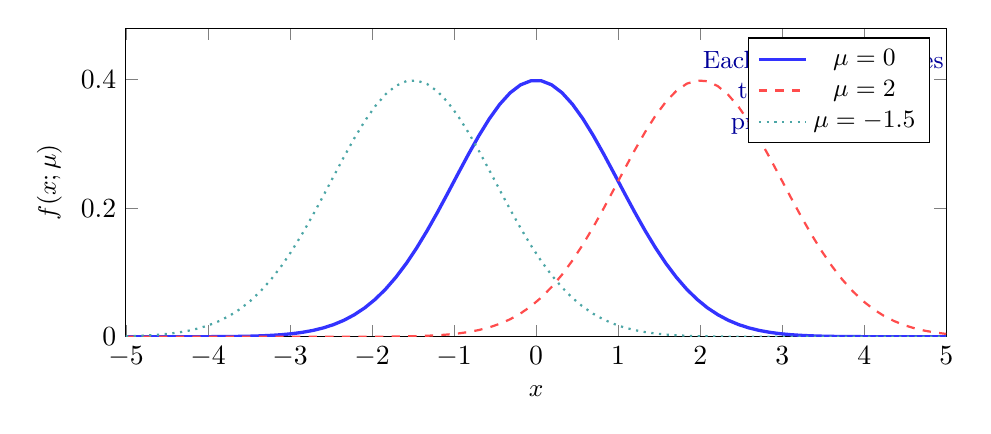
\begin{tikzpicture}
\begin{axis}[
  width=12cm, height=5.5cm,
  xlabel={$x$}, ylabel={$f(x;\mu)$},
  xlabel style={font=\small},
  ylabel style={font=\small},
  xmin=-5, xmax=5, ymin=0, ymax=0.48,
  legend style={font=\small, at={(0.98,0.97)}, anchor=north east},
  samples=80,
]
\addplot[blue!80, very thick, domain=-5:5]
  {(1/sqrt(2*3.14159))*exp(-x^2/2)};
\addlegendentry{$\mu=0$}

\addplot[red!70, thick, dashed, domain=-5:5]
  {(1/sqrt(2*3.14159))*exp(-(x-2)^2/2)};
\addlegendentry{$\mu=2$}

\addplot[teal!70, thick, dotted, domain=-5:5]
  {(1/sqrt(2*3.14159))*exp(-(x+1.5)^2/2)};
\addlegendentry{$\mu=-1.5$}

\node[font=\small, align=center, blue!60!black] at (axis cs: 3.5, 0.38)
  {Each curve integrates\\to 1. These are\\proper densities.};
\end{axis}
\end{tikzpicture}
\end{center}

\subsection{Likelihood slices: fixed $x$, varying $\mu$}

\begin{center}
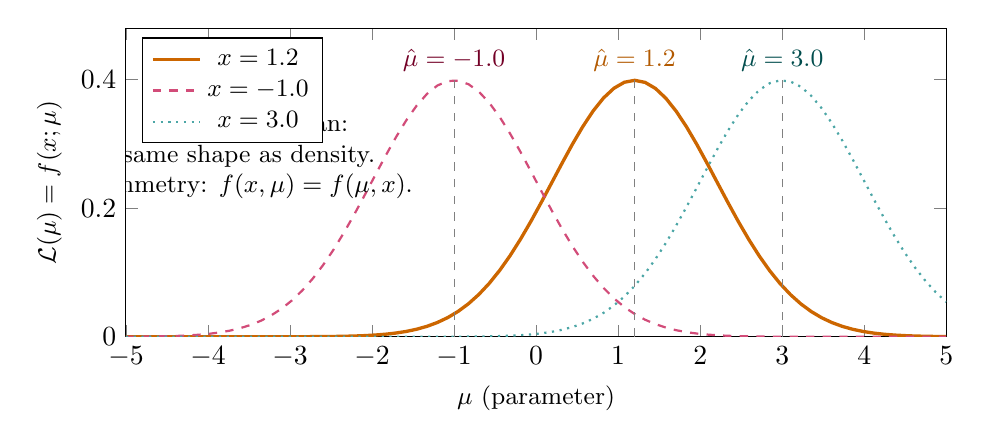
\begin{tikzpicture}
\begin{axis}[
  width=12cm, height=5.5cm,
  xlabel={$\mu$ (parameter)},
  ylabel={$\mathcal{L}(\mu) = f(x;\mu)$},
  xlabel style={font=\small},
  ylabel style={font=\small},
  xmin=-5, xmax=5, ymin=0, ymax=0.48,
  legend style={font=\small, at={(0.02,0.97)}, anchor=north west},
  samples=80,
]
\addplot[orange!80!black, very thick, domain=-5:5]
  {(1/sqrt(2*3.14159))*exp(-(1.2-x)^2/2)};
\addlegendentry{$x=1.2$}

\addplot[purple!70, thick, dashed, domain=-5:5]
  {(1/sqrt(2*3.14159))*exp(-(-1.0-x)^2/2)};
\addlegendentry{$x=-1.0$}

\addplot[teal!70, thick, dotted, domain=-5:5]
  {(1/sqrt(2*3.14159))*exp(-(3.0-x)^2/2)};
\addlegendentry{$x=3.0$}

\draw[dashed, gray] (axis cs: 1.2, 0) -- (axis cs: 1.2, 0.40);
\draw[dashed, gray] (axis cs:-1.0, 0) -- (axis cs:-1.0, 0.40);
\draw[dashed, gray] (axis cs: 3.0, 0) -- (axis cs: 3.0, 0.40);

\node[font=\small, orange!70!black] at (axis cs: 1.2, 0.43)
  {$\hat\mu=1.2$};
\node[font=\small, purple!60!black] at (axis cs:-1.0, 0.43)
  {$\hat\mu=-1.0$};
\node[font=\small, teal!60!black] at (axis cs: 3.0, 0.43)
  {$\hat\mu=3.0$};

\node[font=\small, align=center] at (axis cs: -3.5, 0.28)
  {For the Gaussian:\\same shape as density.\\Symmetry: $f(x,\mu)=f(\mu,x)$.};
\end{axis}
\end{tikzpicture}
\end{center}

Key point: each likelihood curve peaks exactly at
$\hat\mu = x$ (the vertical dashed lines).  The MLE is the
observed value --- trivially, with one observation.

%------------------------------------------------------------
\section{The log-likelihood surface}
%------------------------------------------------------------

Working with $\log f(x,\mu)$ is more convenient.
For the Gaussian:
\[
  \log f(x,\mu)
  = -\frac{(x-\mu)^2}{2} - \frac{1}{2}\log(2\pi).
\]

\begin{center}
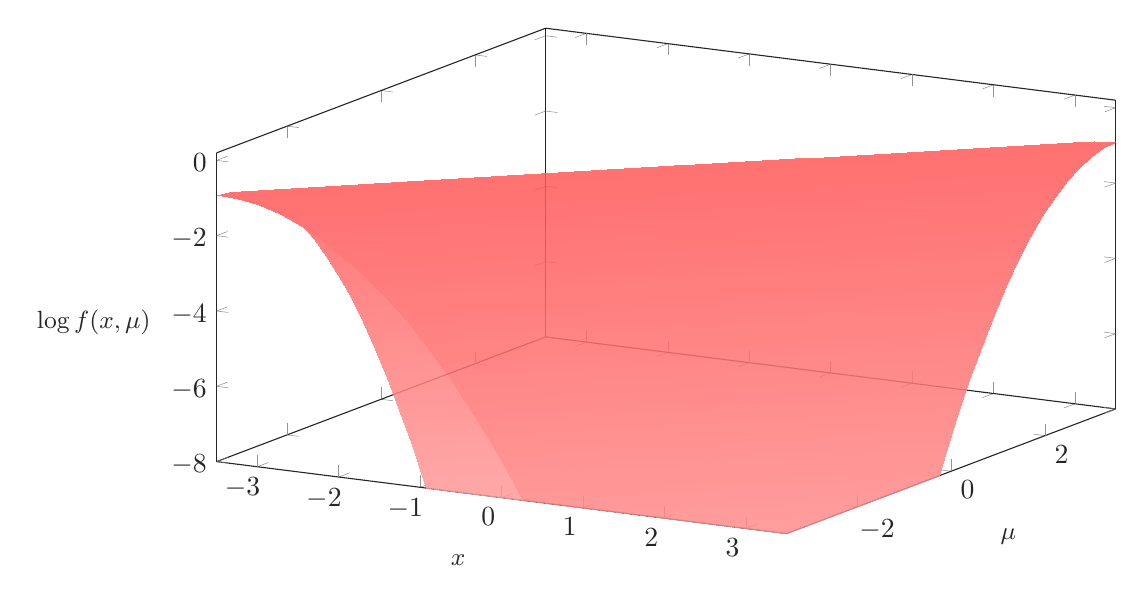
\begin{tikzpicture}
\begin{axis}[
  width=13cm, height=8cm,
  view={30}{25},
  xlabel={$x$},
  ylabel={$\mu$},
  zlabel={$\log f(x,\mu)$},
  xlabel style={font=\small},
  ylabel style={font=\small},
  zlabel style={font=\small, rotate=-90},
  zmin=-8, zmax=0.2,
  colormap={reds}{
    color(0)=(red!5!white)
    color(100)=(red!65)
  },
  shader=interp,
  surf,
  samples=28,
  domain=-3.5:3.5,
  y domain=-3.5:3.5,
  opacity=0.85,
]
\addplot3 [surf, colormap name=reds]
  { -(x-y)^2/2 - 0.919 };
\end{axis}
\end{tikzpicture}
\end{center}

\begin{remark}[The log-likelihood is a paraboloid]
$\log f(x,\mu) = -\tfrac{1}{2}(x-\mu)^2 + \mathrm{const}$
is a downward paraboloid in $(x,\mu)$ space, symmetric
about the diagonal $x = \mu$.
Its ridge is the diagonal: for each fixed $x$, the maximum
over $\mu$ is at $\mu = x$.
This is the geometric reason the Gaussian MLE is the sample mean.
\end{remark}

%------------------------------------------------------------
\section{The Bernoulli case: two separate parametrizations}
%------------------------------------------------------------

\begin{remark}[Two fences live in different spaces]
The triangular fences and the sigmoidal fences cannot share
the same horizontal axis.  Their supports are fundamentally
different:
\begin{itemize}
  \item Triangular fences: parameter $p \in (0,1)$ ---
    the probability itself, bounded.
  \item Sigmoidal fences: parameter $\eta \in \R$ ---
    the linear predictor, unbounded.
\end{itemize}
They are two \emph{parametrizations of the same model},
connected by the logit bijection:
\[
  \eta = \mathrm{logit}(p) = \log\frac{p}{1-p},
  \qquad
  p = \mathrm{expit}(\eta) = \frac{1}{1+e^{-\eta}}.
\]
No linear rescaling of one axis produces the other.
Each deserves its own figure.
\end{remark}

\subsection{Figure 1: $p$-parametrization --- triangular fences}

$f(x,p) = p^x(1-p)^{1-x}$, parameter $p \in (0,1)$.

\begin{center}
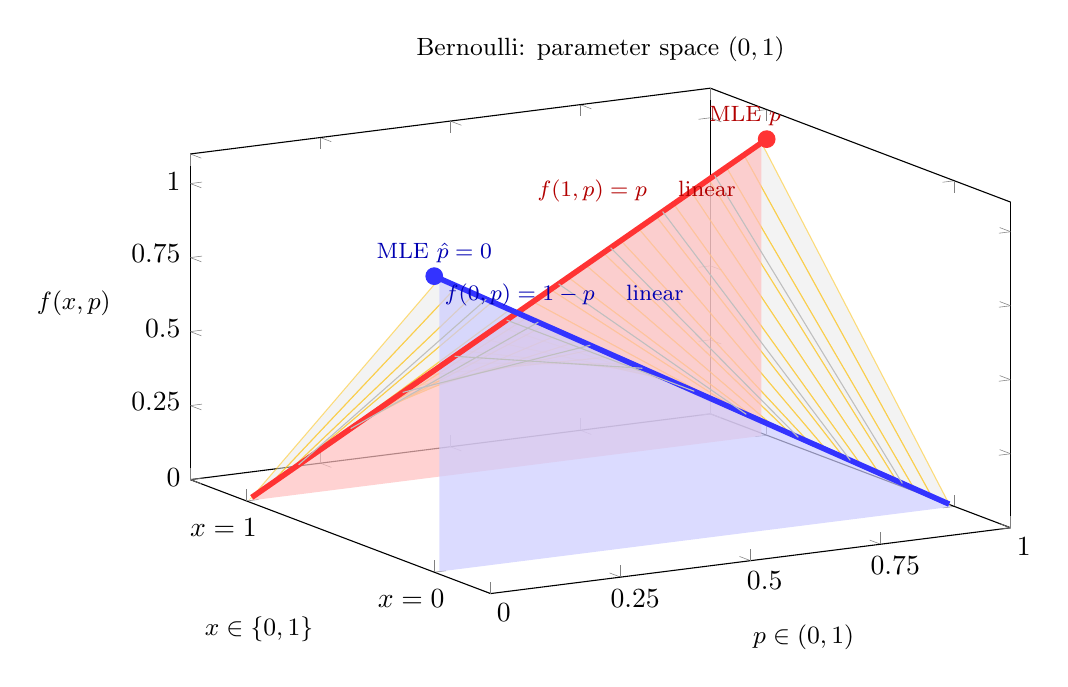
\begin{tikzpicture}
\begin{axis}[
  width=12cm, height=8cm,
  view={-30}{22},
  xlabel={$p \in (0,1)$},
  ylabel={$x \in \{0,1\}$},
  zlabel={$f(x,p)$},
  xlabel style={font=\small},
  ylabel style={font=\small},
  zlabel style={font=\small, rotate=-90},
  xmin=0, xmax=1, ymin=-0.3, ymax=1.3, zmin=0, zmax=1.1,
  xtick={0,0.25,0.5,0.75,1},
  ytick={0,1},
  yticklabels={$x=0$, $x=1$},
  ztick={0,0.25,0.5,0.75,1},
  title style={font=\small},
  title={Bernoulli: parameter space $(0,1)$},
]
\addplot3[surf, shader=flat, fill=gray!18, draw=none, opacity=0.5,
  domain=0.01:0.99, y domain=0:1, samples=30, samples y=2,
] (x, y, {y*x + (1-y)*(1-x)});
\addplot3[fill=red!25, draw=none, opacity=0.7,
  domain=0.01:0.99, samples=60,
] (x, 1, x) \closedcycle;
\addplot3[fill=blue!20, draw=none, opacity=0.7,
  domain=0.01:0.99, samples=60,
] (x, 0, 1-x) \closedcycle;
\addplot3[red!80, very thick, line width=2pt,
  domain=0.01:0.99, samples=60,
] (x, 1, x);
\addplot3[blue!80, very thick, line width=2pt,
  domain=0.01:0.99, samples=60,
] (x, 0, 1-x);
\foreach \pp in {0.1,0.2,...,0.9}{
  \addplot3[gray!50, thin] coordinates {
    (\pp,0,{1-\pp}) (\pp,1,\pp)
  };
}
\addplot3[only marks, mark=*, mark size=3pt, red!80]
  coordinates {(1,1,1)};
\addplot3[only marks, mark=*, mark size=3pt, blue!80]
  coordinates {(0,0,1)};
\node[font=\footnotesize,red!70!black]
  at (axis cs:0.75,1,0.88){$f(1,p)=p$ \quad linear};
\node[font=\footnotesize,blue!70!black]
  at (axis cs:0.25,0,0.88){$f(0,p)=1-p$ \quad linear};
\node[font=\footnotesize,red!70!black]
  at (axis cs:1.0,1,1.08){MLE $\hat p=1$};
\node[font=\footnotesize,blue!70!black]
  at (axis cs:0.0,0,1.08){MLE $\hat p=0$};
\end{axis}
\end{tikzpicture}
\end{center}

The fences are \emph{linear} (triangular) because
$f(1,p)=p$ and $f(0,p)=1-p$ are linear in $p$.
The MLE has no interior maximum: it hits the boundary
$\hat p \in \{0,1\}$.

\begin{remark}[Geometry: hyperbolic paraboloid]
\label{rem:saddle}
The connecting surface is
$z(p,y) = 1 - p - y + 2yp$, a bilinear form,
i.e.\ a \textbf{hyperbolic paraboloid} (saddle surface).
It is a ruled surface: both the vertical grey bars
(fixed $p$, vary $y$) and the lines of constant $y$
(fixed $y$, vary $p$) are straight lines lying exactly
on the surface.
\texttt{pgfplots} with \texttt{samples y=2} renders
this exactly --- no approximation.
The interpolation $y \in [0,1]$ is a visual aid only;
$y \in \{0,1\}$ in the probability model.
\end{remark}

\subsection{Reparametrization bridge}

The logit map $\eta = \log\frac{p}{1-p}$ is a bijection
$(0,1) \to \R$.  It stretches the bounded $p$-axis into
the unbounded $\eta$-axis, compressing the centre
($p \approx 0.5$, $\eta \approx 0$) and expanding the
tails:

\begin{center}
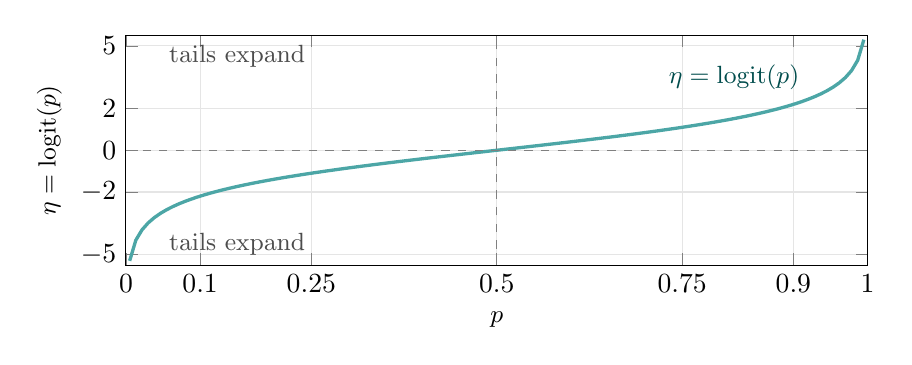
\begin{tikzpicture}
\begin{axis}[
  width=11cm, height=4.5cm,
  xlabel={$p$}, ylabel={$\eta=\mathrm{logit}(p)$},
  xlabel style={font=\small},
  ylabel style={font=\small},
  xmin=0, xmax=1, ymin=-5.5, ymax=5.5,
  xtick={0,0.1,0.25,0.5,0.75,0.9,1},
  ytick={-5,-2,0,2,5},
  samples=120,
  grid=both,
  grid style={gray!20},
]
\addplot[teal!70, very thick, domain=0.005:0.995]
  {ln(x/(1-x))};
\draw[dashed, gray] (axis cs:0.5,-5.5) -- (axis cs:0.5,5.5);
\draw[dashed, gray] (axis cs:0,-0) -- (axis cs:1,0);
\node[font=\small, teal!60!black] at (axis cs:0.82,3.5)
  {$\eta=\mathrm{logit}(p)$};
\node[font=\small, gray!60!black] at (axis cs:0.15,4.5)
  {tails expand};
\node[font=\small, gray!60!black] at (axis cs:0.15,-4.5)
  {tails expand};
\end{axis}
\end{tikzpicture}
\end{center}

Under this map the \emph{linear} fence $f(1,p)=p$
becomes the \emph{sigmoidal} fence
$f(1,\eta)=\mathrm{expit}(\eta)$, and the linear
fence $f(0,p)=1-p$ becomes
$f(0,\eta)=\mathrm{expit}(-\eta)$.
This is not a new model --- it is the same Bernoulli
pmf, expressed in a different coordinate.

\subsection{Figure 2: $\eta$-parametrization --- sigmoidal fences}

$f(y,\eta) = \mathrm{expit}(\eta)^y\,\mathrm{expit}(-\eta)^{1-y}$,
parameter $\eta \in \R$.
This is the likelihood surface of logistic regression
(one observation, varying the linear predictor).

\begin{center}
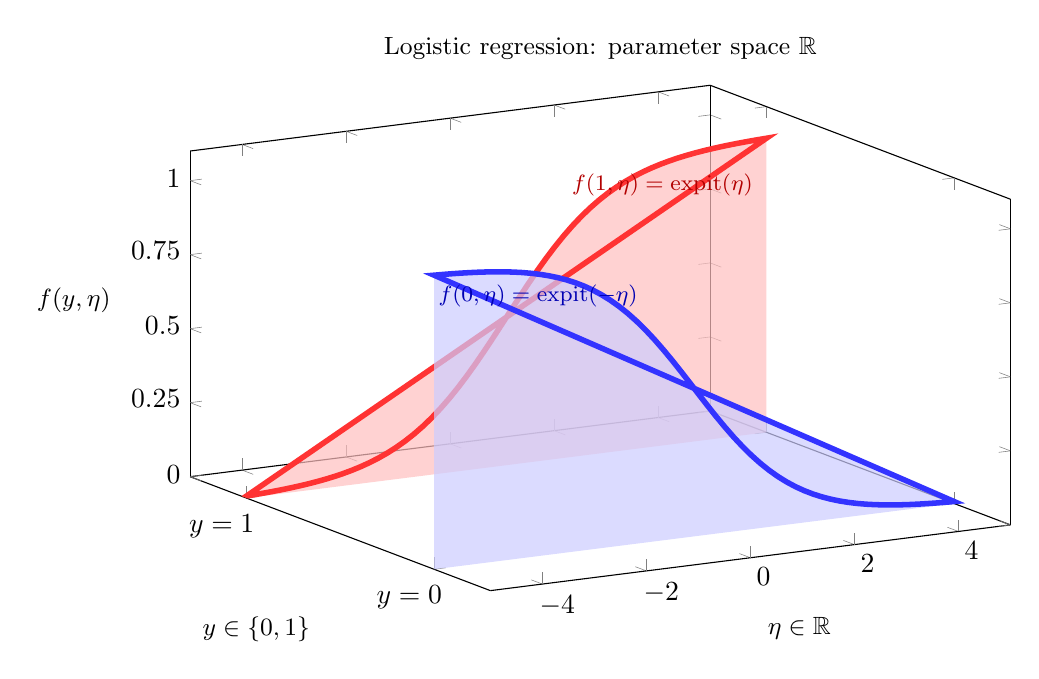
\begin{tikzpicture}
\begin{axis}[
  width=12cm, height=8cm,
  view={-30}{22},
  xlabel={$\eta \in \mathbb{R}$},
  ylabel={$y \in \{0,1\}$},
  zlabel={$f(y,\eta)$},
  xlabel style={font=\small},
  ylabel style={font=\small},
  zlabel style={font=\small, rotate=-90},
  xmin=-5, xmax=5, ymin=-0.3, ymax=1.3, zmin=0, zmax=1.1,
  xtick={-4,-2,0,2,4},
  ytick={0,1},
  yticklabels={$y=0$, $y=1$},
  ztick={0,0.25,0.5,0.75,1},
  samples=60,
  title style={font=\small},
  title={Logistic regression: parameter space $\mathbb{R}$},
]
% Red sigmoidal fence: y=1
\addplot3[fill=red!25, draw=none, opacity=0.7,
  domain=-5:5, samples=60,
] (x, 1, {1/(1+exp(-x))}) \closedcycle;
\addplot3[red!80, very thick, line width=2pt,
  domain=-5:5, samples=60,
] (x, 1, {1/(1+exp(-x))});

% Blue sigmoidal fence: y=0
\addplot3[fill=blue!20, draw=none, opacity=0.7,
  domain=-5:5, samples=60,
] (x, 0, {1/(1+exp(x))}) \closedcycle;
\addplot3[blue!80, very thick, line width=2pt,
  domain=-5:5, samples=60,
] (x, 0, {1/(1+exp(x))});

\node[font=\footnotesize, red!70!black]
  at (axis cs: 3, 1, 0.88){$f(1,\eta)=\mathrm{expit}(\eta)$};
\node[font=\footnotesize, blue!70!black]
  at (axis cs: -3, 0, 0.88){$f(0,\eta)=\mathrm{expit}(-\eta)$};
\end{axis}
\end{tikzpicture}
\end{center}

The fences are now \emph{sigmoidal} because $\mathrm{expit}$
is the inverse logit.  The MLE has no boundary problem:
with $n$ observations the log-likelihood
$\sum_i [y_i\eta_i - \log(1+e^{\eta_i})]$ is strictly
concave in $\boldsymbol\beta$, so the score equation
has a unique interior solution.

\begin{remark}[Geometry: ruled but not saddle]
The connecting surface is
$z(\eta,y) = y\,\mathrm{expit}(\eta)
           + (1-y)\,\mathrm{expit}(-\eta)$.
It is again a ruled surface (linear in $y$ for every
fixed $\eta$), but \emph{not} a hyperbolic paraboloid:
the $\eta$-direction curves sigmoidally, not linearly.
As in Figure~1, \texttt{pgfplots} renders it exactly
(linear in $y$, arbitrary in $\eta$, so \texttt{samples
y=2} suffices).
\end{remark}



%------------------------------------------------------------
\section{What the surface reveals about MLE geometry}
%------------------------------------------------------------

Reading the surface $f(x,\theta)$ as a function of two variables
gives a unified picture:

\begin{enumerate}
  \item \textbf{Density slices} ($\theta$ fixed, $x$ varies):
    cross-sections parallel to the $x$-axis.
    Each must integrate (or sum) to 1 over $\mathcal{X}$.

  \item \textbf{Likelihood slices} ($x$ fixed, $\theta$ varies):
    cross-sections parallel to the $\theta$-axis.
    Their heights are not normalised.
    The \emph{shape} encodes how much each $\theta$ is
    supported by the observed $x$.

  \item \textbf{The ridge} of the surface (maximum over $\theta$
    for each fixed $x$): this is the MLE as a function of $x$.
    For the Gaussian it is the diagonal $\hat\mu(x) = x$.

  \item \textbf{Curvature of the likelihood slice} at $\hat\theta$:
    this is related to Fisher information.
    A sharply curved (narrow) peak means high information ---
    the data localise $\theta$ well.
    A flat peak means low information.
\end{enumerate}

\bigskip
\noindent
The next step (v3): aggregate $n$ independent observations.
The log-likelihood surface becomes a sum, the ridge sharpens,
and the MLE converges to the truth with variance
$1/(n\,\mathcal{I}(\theta))$.

\end{document}
